\documentclass[a4paper,norsk,12pt]{book}
\usepackage[norsk]{babel}
\usepackage[utf8]{inputenc}
\usepackage{enumitem}
\usepackage{amsmath}
\usepackage{color}
\usepackage{icomma}
\def\d{\ensuremath{\mathrm{d}}}
\def\ex{\ensuremath{\hat{e}_x}}
\def\ey{\ensuremath{\hat{e}_y}}
\def\ez{\ensuremath{\hat{e}_z}}
\def\er{\ensuremath{\hat{e}_r}}
\def\eth{\ensuremath{\hat{e}_\theta}}

\newcommand{\unit}[1]{~\mathrm{#1}}
\newcommand{\ans}[1]{\underline{\underline{#1}}}

\usepackage[svgnames]{xcolor}
\usepackage[most]{tcolorbox}
\usetikzlibrary{shadows}

\newcounter{exa}

\tcbset{
myexample/.style={
  enhanced,
  colback=blue!10!white,
  colframe=black,
  fonttitle=\scshape,
  titlerule=0pt,
  title={\refstepcounter{exa}Eksempel~\theexa},
  title style={fill=blue!40!white},
  coltitle=black,
  drop shadow,
  highlight math style={reset,colback=LightBlue!50!white,colframe=Navy}
  }
}

\newtcolorbox{texample}{myexample}


\begin{document}
\tableofcontents

\chapter{Enheter}
I fysikk har de fleste størrelsene enheter. Enheten er en essensiell del av størrelsen, så hvis om vi oppgir bare tallverdien er ikke størrelsen tilstrekkelig spesifisert. For eksempel er det ikke tilstrekkelig å si at en stav er 1 lang. Da blir det bare gjetting om det er 1 meter, 1 fot eller noe helt annet.\footnote{Mars-sonden Mars Climate Orbiter kræsjlandet fordi programvaren ga resulter i pundsekunder (lbf s), mens resultatene ble tolket som Newtonsekunder(Ns) som var det kontrakten mellom NASA og Lokheed hadde spesifisert at skulle brukes.} Når vi regner med størrelser som har enheter er enhetene en del av utregningen, og vi tar de med også i alle mellomregninger.

Ved å ta med enheter hele veien gjennom beregningen får vi automatisk en kontroll på om beregningen vi har utført er fornuftig. Hvis vi skal regne ut en energi og ender opp med enhet $\mathrm{m^2/s^2}$ vet vi at det er noe feil i utreningen. Enhetene kan også hjelpe oss å huske hvordan vi formler ser ut. Hvis vi for eksempel husker at vi ut fra en hastighet (m/s) og en tid (s) kan finne avstanden, men ikke hvordan de skal kombineres kan vi straks se dette ut fra enhetene. Den eneste måten å kombinere m/s og s til å gi riktig enhet for lengde (m) er å multiplisere de sammen. Altså må vi ha $x = vt$.

Det finnes mange forskjellige enhets-systemer. Det mest brukte, og det eneste som blir diskutert her, er SI-systemet (Système international d'unités). SI-systemet er bygget opp fra syv grunnenheter {\color{red}[Denne beskrivelsen er i ferd med å bli utdatert]}:
\begin{itemize}
\item Lengde - meter (m)
\item Masse - kilogram\footnote{Merk at det er kilogram som er grunnenheten, ikke gram.} (kg)
\item Tid - sekund (s)
\item Elektrisk strøm - ampere (A)
\item Temperatur - kelvin (K)
\item Stoffmengde - mol (mol)
\item Lysstyrke - candela (cd)
\end{itemize}
Enhetene til alle andre størrelser får man ved å kombinere grunn-enhetene. En del kombinasjoner som ofte opptrer har fått egne navn og symbol. En rekke størrelser og enheter man ofte treffer på i fysikk-oppgaver er listet i tabell \ref{tab:enheter:mekanikk}-\ref{tab:enheter:magnetisme}.

%% Begin tables
\begin{table}[tbp]
{\small
\begin{tabular}{|l|l|l|l|}
\hline
\hline
{\bf Størrelse} & {\bf Symbol} & {\bf Enhet} & {\bf Navn på enhet} \\
\hline
Posisjon & $\vec{x}, \vec{r}$ & 1~m & Meter \\
Hastighet & $\vec{v}$ &  1~m/s & \\
Akselerasjon & $\vec{a}$ & $1~\mathrm{m/s^2}$ & \\
\hline
Masse  & $m$ & 1~kg & Kilogram \\
Massetetthet, masse per volum & $\rho$ & $1~\mathrm{kg/m^3}$ & \\
\hline
Energi & $E, K, U$ & 1 J = 1 Nm = 1 $\mathrm{kg m^2/s^2}$ & Joule \\
Arbeid & $W$ & 1 J & \\
Effekt & $P$ & 1 W = 1 J/s & Watt \\
\hline
Kraft & $\vec{F}$ & 1 N = 1 $\mathrm{kg m/s^2}$ & Newton \\
Bevegelsesmengde & $\vec{p}, \vec{P} $ & 1 $\mathrm{kg m/s^2}$ & \\
Impuls, støt & $\vec{J}$ & $\mathrm{1~Ns = 1~kg m/s^2}$ & \\
\hline
\hline
\end{tabular}
}
\caption{Størrelser og enheter først og fremst knyttet til mekanikk, men energi, arbeid og effekt er også viktig i andre deler av fysikken.}
\label{tab:enheter:mekanikk}
\end{table}

\begin{table}[tbp]
{\small
\begin{tabular}{|l|l|l|l|}
\hline
\hline
{\bf Størrelse} & {\bf Symbol} & {\bf Enhet} & {\bf Navn på enhet} \\
\hline
Ladning & $Q, q$ & 1 C & Coulomb \\
Ladningstetthet, ladning per lengde & $\lambda$ & 1 C/m  & \\
Ladningstetthet, ladning per areal & $\sigma$ & 1 C/m$^2$ & \\
Ladningstetthet, ladning per volum & $\rho$ & 1 C/m$^3$ & \\
\hline
Elektrisk strøm & $I, i$ & 1 A = 1 C/s & Ampere \\
Elektrisk strømtetthet & $\vec{J}$ & 1 A/m$^2$ & \\
\hline
Elektrisk felt & $\vec{E}$ & 1 N/C = 1 V/m & \\
Elektrisk fluks & $\Phi_E$ & 1 Nm$^2$/C = 1 Vm & \\
\hline
Elektrisk potensial & $V$ & 1 V = 1 J/C & Volt \\
Elektromotorisk spenning & ${\cal E}$ & 1 V & \\
\hline
Motstand, resistans & $R, r$ & 1 $\Omega$ = 1 V/A & Ohm \\
Resisitivitet & $\rho$ & 1 $\Omega$m & \\
Konduktivitet & $\sigma$ & 1 $(\Omega\mathrm{m})^{-1}$ & \\
\hline
Kapasitans & $C$ & 1 F = C/V & Farad \\
\hline
\hline
\end{tabular}
}
\caption{Størrelser og enheter knyttet til elektriske fenomen.}
\label{tab:enheter:elektrisk}
\end{table}

\begin{table}[tbp]
{\small
\begin{tabular}{|l|l|l|l|}
\hline
\hline
{\bf Størrelse} & {\bf Symbol} & {\bf Enhet} & {\bf Navn på enhet} \\
\hline
Magnetisk felt & $\vec{B}$ & $1~\mathrm{T} = 1~\mathrm{N/Am}$ & Tesla \\
Magnetisk fluks & $\Phi_{B}$ & $1~\mathrm{Wb} = 1~\mathrm{Tm^2}$ & Weber \\
Magnetisering  & $\vec{M}$ & 1 A/m & \\
Induktans & $L$ & 1 H = 1 Wb/A = 1 Vs/A & Henry\\
Gjensidig induktans & $M$ & 1 H & \\
\hline
\hline
\end{tabular}
}
\caption{Størrelser og enheter knyttet til magnetiske fenomen.}
\label{tab:enheter:magnetisme}
\end{table}
%% End tables


\chapter{Skalarer og vektorer}
En del fysiske størrelser kan spesifiseres fullstendig ved hjelp av et tall + enhet. Dette er en skalar. Merk at den skalare størrelsen kan ha samme verdi på alle punkter i rommet (eksempel: lysets hastighet i vakuum) eller variere fra sted til sted (eksempel: temperatur). Skalare størrelser kan også endre seg med tiden. Når vi regner med skalarer kan vi bruke alle de vanlige regneartene.

Andre fysiske størrelser er ikke fullstendig spesifisert ved hjelp av bare et tall + enhet. For eksempel holder det ikke å si at det blåser $10~\mathrm{m/s}$ -- vi vil som regel vite retningen også. En størrelse som må spesifiseres både ved hjelp av verdi og retning kalles en vektor. 


\section{Vektoroperasjoner}
Akkurat som skalarer kan vektorer ha samme verdi og retning i alle punkter i rommet, eller verdi og/eller retning kan variere fra punkt til punkt. Verdi og retning kan også endre seg med tiden. For vektorer har vi i tillegg til addisjon og subtraksjon tre typer multiplikasjon:
\begin{itemize}
\item Multiplikasjon med en skalar $\to$ gir en vektor som svar
\item Indreprodukt/prikkprodukt mellom to vektorer $\to$ gir en skalar som svar
\item Vektorprodukt/kryssprodukt mellom to vektorer $\to$ gir en vektor som svar
\end{itemize}

\section{Enhetsvektorer}
Når vi jobber med vektorstørrelser er det ofte nyttig å introdusere en eller flere \emph{enhetsvektorer}. En enhetsvektor er ganske enkelt en vektor med lengde 1, og nytten av den er at den peker i en bestemt retning. Mer at selv når vi jobber med vektorfelt som har dimensjon (f.eks. m/s eller N/C) er enhetsvektoren dimensjonsløs. Vanligvis bruker vi enhetsvektorer som peker i retningene til aksene i koordinatsystemet vårt, f.eks. i $x$-, $y$-, og $z$-retning. Dette blir diskutert i mer detalj nedenfor. Noen ganger ønsker vi imidlertid å bruke en enhetsvektor som peker i samme retning som en vilkårlig vektor. Hvis vi for eksempel har en posisjonsvektor $\vec{r}$ kan det noen ganger være nyttig å skrive den som 
\begin{equation}
	\vec{r} = r \hat{r}
	\label{eq:vektorer:r}
\end{equation}
der $r$ er lengden av vektoren, altså $r = |\vec{r}|$ og $\hat{r}$ er en enhetsvektor som peker i samme retning som $\vec{r}$. Ved å se på ligning (\ref{eq:vektorer:r}) finner vi ut at enhetsvektoren kan finnes fra vectoren $\vec{r}$ som
\begin{displaymath}
	\hat{r} = \frac{\vec{r}}{|\vec{r}|}.
\end{displaymath}

\subsection{Enhetsvektorer i et kartesisk koordinatsystem}
Vi ser nå på et vanlig kartesisk koordinatsystem, altså et koordinatsystem som består av en $x$-, $y-$ og $z$-akse som står normalt på hverandre. Vi vet da at enhver vektor kan dekomponeres i $x$-, $y$- og $z$-komponenter. For eksempel kan vektoren $\vec{r}$ skrives som $(r_x, r_y, r_z)$ der vi har listet opp hver enkelt komponent. Ofte er det nyttigere å bruke en notasjon der vi multipliserer hver komponent med enhetsvektoren som går i den aktuelle retningen:
\begin{displaymath}
\begin{aligned}
	\vec{r} &= r_x\hat{\i} + r_y\hat{\j} + r_z\hat{k} \\
	&= r_x\ex + r_y\ey + r_z\ez.
\end{aligned}
\end{displaymath}
Den eneste forskjellen på de to linjene her er at det er brukt uliknotasjon for enhetsvektorene. Begge notasjonene er i vanlig bruk, så det er nødvendig å kjennet til begge. I denne teksten velger jeg å bruke $\ex, \ey, \ez$ fordi notasjonen viser eksplisitt hvilken retning hver enhetsvektor peker, og fordi den er helt tilsvarende den mest brukte notasjonen for sylinder- og sfæriske koordinater.

Det er nyttig å kjenne resultatet av prikk- og kryssprodukt mellom de ulike enhetsvektorene, fordi det er da enkelt å regne ut prikk- eller kryssprodukt mellom to vilkårlige vektorer som er uttrykt ved hjelp av enhetsvektorene. Siden alle enhetsvektorene har lengde 1 og står normalt på hverandre er prikk-produktet svært enkelt:
\begin{displaymath}
	\hat{e}_i \cdot \hat{e}_j = 
	\left\{
		\begin{aligned}
		1 \text{ hvis } i = j \\
		0 \text{ hvis } i\neq j
		\end{aligned}
	\right.
	\label{eq:vektor:prikkprodukt}
\end{displaymath}
der $i$ og $j$ kan være enten $x, y$ eller $z$. Kryssproduktet mellom enhetsvektorene er litt mer komplisert, men kan relativt enkelt finnes ved hjelp av høyrehåndsregelen. Siden alle enhetsvektorene har lengde 1 og står normalt på hverandre blir også kryssproduktet en vektor med lengde 1, bortsett fra hvis vi tar kryssprodukt av en enhetsvektor med seg selv---da får vi 0.
\begin{displaymath}
\begin{aligned}
	\ex\times\ex &= \ey\times\ey = \ez\times\ez = 0 \\
	\ex \times \ey & = \ez \\
	\ex \times \ez & = -\ey \\
	\ey \times \ez &= \ex 
	\label{eq:vektor:kryssprodukt}
\end{aligned}
\end{displaymath}
Hvis enhetsvektorene kommer i annen rekkefølge bruker vi den generelle regelen for kryssprodukt som gjelder for alle vektorer, inkludert enhetsvektorer, 
\begin{displaymath}
	\vec{a}\times\vec{b} = -\vec{b}\times\vec{a}
\end{displaymath}

\subsubsection{Regneeksempel}
Vi har hastighetsvektoren
\begin{displaymath}
	\vec{v} = (1~\mathrm{m/s})\ex - (3~\mathrm{m/s})\ey + (2~\mathrm{m/s})\ez
\end{displaymath}
og magnetfeltvektoren 
\begin{displaymath}
	\vec{B} = (1.2~\mathrm{T})\ex + (0.5~\mathrm{T})\ey - (0.7~\mathrm{T})\ez.
\end{displaymath}
Vi kan nå bruke relasjonene (\ref{eq:vektor:prikkprodukt}) og (\ref{eq:vektor:kryssprodukt}) til å regne ut prikk- og kryss-produktet av $\vec{v}$ og $\vec{B}$\footnote{$\vec{v}\times\vec{B}$ er et produkt som det ofte er behov for å beregne når man jobber med magnetiske krefter. $\vec{v}\cdot\vec{B}$ er ikke et produkt som vanligvis opptrer i fysiske beregninger, men det er ingenting som hindrer oss i å beregne dette produktet.}. Merk at beregningene her gjøres litt ekstra omstendelig---vanligvis vil man ikke skrive opp de leddene som gir 0 i det hele tatt, men for å vise mest mulig detaljer er alle ledd med her.
\begin{displaymath}
\begin{aligned}
	\vec{v}\cdot\vec{B} &= \left[ (1~\mathrm{m/s})\ex - (3~\mathrm{m/s})\ey + (2~\mathrm{m/s})\ez \right] \cdot
	\left[(1.2~\mathrm{T})\ex + (0.5~\mathrm{T})\ey - (0.7~\mathrm{T})\ez\right] \\
	&= (1.2~\mathrm{Tm/s})\ex\cdot\ex + (0.5~\mathrm{Tm/s})\ex\cdot\ey -  (0.7~\mathrm{Tm/s})\ex\cdot\ez \\
	&\quad- (3.6~\mathrm{Tm/s})\ey\cdot\ex- (1.5~\mathrm{Tm/s})\ey\cdot\ey+ (2.1~\mathrm{Tm/s})\ey\cdot\ez \\
	&\quad+ (2.4~\mathrm{Tm/s})\ez\cdot\ex+ (1.0~\mathrm{Tm/s})\ez\cdot\ey -  (1.4~\mathrm{Tm/s})\ez\cdot\ez \\
	&= 1.2~\mathrm{Tm/s} - 1.5~\mathrm{Tm/s} - 1.4~\mathrm{Tm/s} \\
	&= -1.7~\mathrm{Tm/s}.
\end{aligned}
\end{displaymath}
\begin{displaymath}
\begin{aligned}
	\vec{v}\times\vec{B} &= \left[ (1~\mathrm{m/s})\ex - (3~\mathrm{m/s})\ey + (2~\mathrm{m/s})\ez \right] \times
	\left[(1.2~\mathrm{T})\ex + (0.5~\mathrm{T})\ey - (0.7~\mathrm{T})\ez\right] \\
	&= (1.2~\mathrm{Tm/s})\ex\times\ex + (0.5~\mathrm{Tm/s})\ex\times\ey -  (0.7~\mathrm{Tm/s})\ex\times\ez \\
	&\quad- (3.6~\mathrm{Tm/s})\ey\times\ex- (1.5~\mathrm{Tm/s})\ey\times\ey+ (2.1~\mathrm{Tm/s})\ey\times\ez \\
	&\quad+ (2.4~\mathrm{Tm/s})\ez\times\ex+ (1.0~\mathrm{Tm/s})\ez\times\ey -  (1.4~\mathrm{Tm/s})\ez\times\ez \\
	&=(0.5~\mathrm{Tm/s}+3.6~\mathrm{Tm/s})\ex\times\ey + (-0.7~\mathrm{Tm/s}-2.4~\mathrm{Tm/s})\ex\times\ez \\
	&\quad+(2.1~\mathrm{Tm/s}-1.0~\mathrm{Tm/s})\ey\times\ez \\
	&=(4.1~\mathrm{Tm/s})\ez - (3.1~\mathrm{Tm/s})(-\ey) +(1.1~\mathrm{Tm/s})\ex \\
	&=(1.1~\mathrm{Tm/s})\ex + (3.1~\mathrm{Tm/s})\ey + (4.1~\mathrm{Tm/s})\ez
\end{aligned}
\end{displaymath}

\subsection{Enhetsvektorer i sylinderkoordinater}
Enhver bevegelse \emph{kan} beskrives ved hjelp av kartesiske koordinater, men noen bevegelse vil da se unødvendig komplisert ut. Dette gjelder blant annet sirkelbevegelser og skurebevegelser. Disse bevegelsene beskrivers bedre i sylinderkoordinater. Vi har da
\begin{itemize}
\item
 en koordinat som beskriver avstanden fra sentrum av bevegelsen. Denne koordinaten kalles ofte $r$.
\item
 en koordinat som beskriver vinkelen relativt til en (tilfeldig valgt) retning i planet der sirkelbevegelsen skjer. Denne koordinaten kalles ofte $\theta$.
\item
en koordinat som beskriver høyden over det planet vi tok utgangspunkt i. Denne koordinaten kalles ofte $z$. 
\end{itemize}
Vi definerer nå tre enhetsvektorer $\er, \eth$ og $\ez$. Enhetsvektoren $\ez$ er akkurat slik som enhetsvektorene diskutert i forbindelse med de kartesiske koordinatene, men de to andre er litt annerledes: $\er$ og $\eth$ peker nemlig i ulik retning avhengig av hvilket punkt vi ser på. Enhetsvektoren $\er$ peker i samme retning som forbindelseslinjen mellom origo og punktet vi ser på, mens $\eth$ står $90^\circ$ på $\er$ og $\eth$ med retningen bestemt slik at $\er, \eth$ og $\ez$ utgjør et høyrehendt system når de er tatt i den rekkefølgen. Dette betyr at når $z$-aksen peker oppover øker vinkelen \emph{mot} klokken. Vi kan nå uttrykke en vilkårlig vektor ved hjelp av enhetsvektorene vi har definert,
\begin{displaymath}
	\vec{a} = a_r\ex + a_\theta\eth + a_z\ez.
\end{displaymath}

Siden retningen til $\er$ og $\eth$ varierer fra punkt til punkt vil de påvirkes av derivasjon. 
\chapter{Derivasjon og integrasjon}

\section{Derivasjon}
\section{Integrasjon}
\section{Differensialligninger}

\chapter{Figurer}
En god figur er nyttig for å organisere opplysningene i en problemstilling før vi begynner å regne. Hva slags figur vi tegner vil avhenge av problemstillingen. Typiske figurer inkluderer:
\begin{enumerate}
\item
	Bevegelsesdiagram (mekanikk)
\item
	Frilegemediagram (mekanikk)
\item
	pV-diagram (termodynamikk)
\end{enumerate}

\section{Bevegelsesdiagram}

\section{Frilegemediagram}
I mekanikk-oppgaver er frilegemediagrammer vanligvis den nyttigste figurtypen. Fokus i et frilegemediagram er hvilke krefter som virker på hver del av systemet vi ser på. Ordet frilegemediagram antyder at vi skal tegne et diagram for hver del (=legeme), men hvis systemet ikke er for komplisert kan det gå greit å tegne på krefter på alle deler i en og samme figur.

Noen tips for et godt frilegemediagram:
\begin{itemize}
\item
Velg et gunstig kooridnatsystem, og tegn dette inn. Et gunstig koordinatsystem er vanligvis et koordinatsystem der ortogonale akser der bevegelsen er parallell med en av aksene.
\item
Alle \emph{relevante} krefter på alle deler av systemet skal tegnes inn. Krefter som kan utelates som irrelevante er de som trivielt summerer til null og ikke skal brukes til noe i beregningen. Hvis du er i tvil om en kraft er relevant---ta den med!
\item
Kreftene skal i hovedsak tegnes inn med riktig angrepspunkt, men noen ganger er det nyttig å forskyve angrepspunktet litt for å gjør diagrammet mer oversiktelig.
\item
Kreftene tegnes inn med riktig retning hvis denne er kjent. Hvis retningen er ukjent tegnes kraften inn med antatt retning---denne vil bekreftes eller korrigeres av beregningen.
\item
Dekomponer krefter som ikke er parallell med aksene i koordinatsystemet du har valgt. Merk av hvilke krefter som er dekomponert for å unngå dobbeltelling.
\item
Tegn gjerne inn fart og/eller akselerasjon i frilegemediagrammet, men tegn disse størrelsene inn på en slik måte at det ikke er fare for å forveksle dem med krefter. 
\end{itemize}

\section{pV-diagram}
I termodynamikk uttykker vi tilstanden til et system ved å spesifisere en rekke ulike variable, f.eks.~trykk, volum, temperatur og stoffmengde. Hvis vi gjør noe med dette systemet---som å varme det opp eller komprimere det---vil \'en eller flere av disse variablene endres. Vi kan se for oss å fremstille denne endringen i et mange-dimensjonalt koordinatsystem, men slike er vanskelig eller umulig å tegne. Derfor er det oftest nyttig å velge ut to av variablene og tegne inn endringen i et to-dimensjonalt koordinatsystem. I veldig mange tilfeller---og praktisk talt alle tilfellene som er aktuelle i grunnleggende fysikk-kurs---er trykk ($p$) og volum ($V$) det nyttigste paret av variabler. Vi tegner da et pV-diagram der trykket varierer langs den horisontale aksen (``$x$-aksen'') og volumet variere langs den vertikale aksen (``$y$-aksen'').

Det som gjør pV-diagram spesielt nyttig er at arbeidet som systemet gjør beregnes som 
\begin{displaymath}
	W = \int_{V_1}^{V_2}p\d V.
\end{displaymath}
Slik pV-diagrammet er definert kan vi altså tolke arealet under grafen som forbinder start- og sluttpunktet som arbeidet systemet gjør (eller blir gjort på systemet). 

Både trykk og volum vil alltid være positive størrelser. Vi ser da at en prosess som beveger seg mot høyre i pV-diagrammet gir positivt arbeid---altså systemet gjør arbeid på omgivelsene. En prosess som beveger seg mot venstre i pV-diagrammet gir negativt arbeid---altså at omgivelsene gjør arbeid på systemet. En prosess som beveger seg rett opp eller rett ned i pV-diagrammet gjør ikke noe arbeid.

Hvis systemet er en ideell gass med konstant stoffmengde er konstant-temperatur-linjer i pV-diagrammet gitt som
\begin{displaymath}
	p = \frac{nRT}{V} = \frac{\text{konstant}}{V}
\end{displaymath}
der konstanten er større, jo større temperaturen er. Dette betyr at punkter nede til venstre har lav temperatur, mens punkter oppe til høyre har høy temperatur.
\chapter{Bevaringslover}
\chapter{Usikkerhet og signifikante sifre}
I motsetning til i matematikk der vi som regel kan anta at vi har eksakt kjennskap til størrelsene vi jobber med har vi i fysikk generelt bare kjennskap til størrelsen med en viss presisjon. Dette skyldes at fysiske størrelser har opphav i målinger og der kan vi aldri ha uendelig presisjon. Skal vi gjøre ting helt korrekt skal størrelsen oppgis sammen med dens estimerte usikkerhet.\footnote{Heller ikke usikkerheten er eksakt bestemt, men det er som regel mulig å estimere denne på en systematisk måte.
} For eksempel kan en lengde oppgis som $x=(1,03\pm0,02)~\mathrm{m}$. Dette betyr det beste estimatet vi har på lengden er $x = 1,03~\mathrm{m}$. Usikkerheten $\pm0,02~\mathrm{m}$ betyr at vi mener å vite at hvis denne lengden blir målt mange ganger vil flesteparten\footnote{Det vanligste er å bruke en definisjon av usikkerheten som gjør at 67\% at målingene skal havne innenfor intervallet definert av usikkerheten.} av målingene skal vise mellom $x=1,01~\mathrm{m}$ og $x=1,05~\mathrm{m}$. 

I regneoppgaver forholder vi oss vanligvis litt mer avslappet til usikkerheten i størrelsene, men vi glemmer den ikke helt. Hvis f.eks. en energi oppgis som $2,52~\mathrm{J}$ tolkes det som at usikkerheten er i det siste sifferet. Det kan altså tenkes at den riktige verdien er $2,51~\mathrm{J}$ eller $2,55~\mathrm{J}$, men sannsynligvis ikke at avviket er så stort at den riktige verdien er $2,60~\mathrm{J}$. En tommelfingerregel for å få en fornuftig presisjon i svaret av en beregning er å ikke ta med flere sifre i sluttsvaret enn det var i den inn-verdien med færrest sifre.

Noen få ord om hvordan man teller sifre: Hvis vi teller fra venstre er det første sifferet som er ulik 0 det første vi teller. Deretter teller alle sifre med i regnskapet. Eksempler:
\begin{itemize}
	\item 1,54 -- tre sifre
	\item 0,03 -- ett siffer
	\item$1,3\times10^6$ -- to sifre
\end{itemize}
Merk at hvis du får svaret $238~\mathrm{m}$ og kun skal ha med to sifre må svaret skrives som $2,4\times10^2~\mathrm{m}$ for å følge denne regelen siden å skrive det avrundete tallet $240~\mathrm{m}$ fremdeles er å skrive tre sifre.


\section{Estimering av usikkerhet}
Noen ganger er ikke tommelfingerregelen om antall signifikante sifre tilstrekkelig. For eksempel må usikkerhet behandles skikkelig hvis man skriver en vitenskaplig artikkel eller en teknisk rapport. Også i labøvinger er det vanlig å kreve at usikkerheten behandles på en ordentlig måte. 

\subsection{Ulike typer usikkerhet}
Det er vanlig å klassifisere måleusikkerhet i to kategorier: systematisk og statistisk. Den systematiske usikkerheten er direkte knyttet til måleinstrumentet eller metoden, og vil typisk gi feil i samme retning---altså for stor eller for liten verdi---hver gang dersom målingen gjentas. Et eksempel finner vi dersom vi skal måle bredden av en planke ved hjelp av en linjal. Den korrekte bredden finner vi dersom linjalen er plassert perfekt i $90\circ$ vinkel over planken. Dersom vinkelen ikke er helt riktig vil vi ende opp med å måle en bredde som er for stor, men det er ingen vinkel som gir for liten bredde. 

Statistisk usikkerhet beskriver det at enhver måling som forsøker å gå til grensen av nøyaktigheten som er mulig å oppnå med det aktuelle måle\-instrumentet alltid vil ha en viss variabilitet som typisk fordeler seg tilfeldig til begge sider av den sanne verdien. I de fleste tilfeller vil denne variasjonen beskrives godt som en gaussisk/standard-fordeling. 

Forholdet mellom systematisk og statistisk usikkerhet kan belyses ved å se på forskjellen mellom \emph{presisjon} og \emph{nøyaktighet} som er illustrert i figur \ref{fig:usikkerhet:presisjon}. Presisjon beskriver hvor godt gjentatte målinger stemmer overens med hverandre, slik at god presisjon henger sammen med en liten statistisk usikkerhet. Nøyaktighet beskriver hvor godt gjennomsnittet av mange målinger treffer den sanne verdien som vi prøver å finne ved hjelp av målingene. Nøyaktighet er derfor knyttet til systematisk usikkerhet. Som figuren viser kan vi ha f.eks. god nøyaktighet, men samtidig dårlig presisjon. Ideellt sett vil vi gjøre både nøyaktigheten og presisjonen så god som mulig, men det har liten verdi å gjøre den ene veldig god dersom den andre er dårlig.

\begin{figure}[htp]
	\begin{center}
		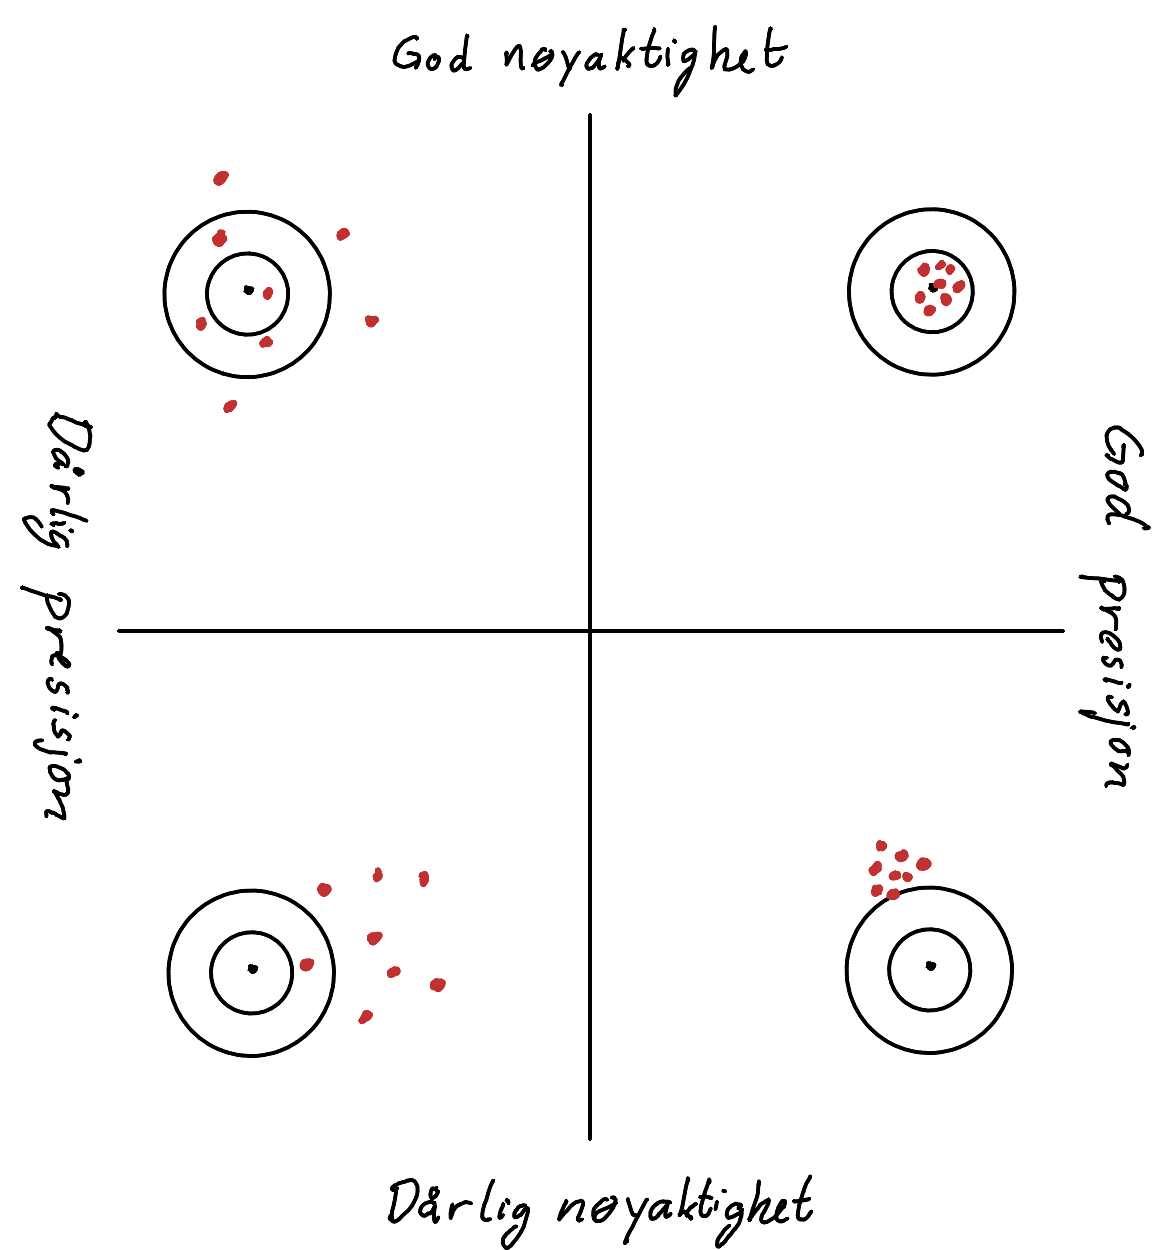
\includegraphics[width=.5\textwidth]{./presisjon}
	\end{center}
	\caption{Illustrasjon av forskjellen mellom begrepene nøyaktighet og presisjon. En god måling ønsker vi at skal være både nøyaktig og presis.}
	\label{fig:usikkerhet:presisjon}
\end{figure}


\subsection{Absolutt og relativ usikkerhet}
Avhengig av sammenhengen brukes to ulike måter å oppgi usikkerheten på: absolutt og relativ usikkerhet. Begge deler uttrykker det samme, det er bare ulike måter å presentere informasjonen på. Dersom vi har en lengde oppgitt som $x=(1,03\pm 0,02)\unit{m}$ da omtaler vi størrelsen $\sigma_x = 0,02\unit{m}$ den \emph{absolutte usikkerheten}. Denne har alltid samme enheter som størrelsen selv. Dersom vi er mer interessert i hvor stor usikkerheten er sammenlignet med den målte størrelsen selv gir vi heller den \emph{relative usikkerheten}: 
\begin{displaymath}
	\frac{\sigma_x}{x} = \frac{0,02\unit{m}}{1,03\unit{m}} = 0,019 = 1,9\%
\end{displaymath}
Siden den relative usikkerheten er et forholdstall har den ingen dimensjon, men oppgis enten som et desimaltall eller som prosent.

Det er ingen egentlige regler for når man skal bruke absolutt og når man skal bruke relativ usikkerhet, men det er mulig å gi noen tommelfingerregler. Hvis man har en enkelt størrelse oppgitt med usikkerhet, er det som regel den absolutte usikkerheten som er enklest å tolke. Dersom man derimot har behov for å sammenligne usikkerheten til målinger av størrelser med ulik benevning er det meningsløst å sammenligne absolutt usikkerhet (hva er størst usikkerhet, $\pm 3\unit{cm}$ eller $\pm 2\unit{^\circ C}$?). Derimot kan en slik sammenligning gjøres meningsfull ved å bruke relativ usikkerhet.

\begin{texample}
{\bf
Vi har $n=(0,022\pm0,001)\unit{mol}$ av en ideell gass i en beholder med volum $V = (5,00\pm0,01)\cdot 10^{-4}\unit{m^3}$. Vi måler trykket til å være $p=(1,035\pm0,011)\cdot 10^5\unit{Pa}$ og ønsker å regne ut temperaturen fra disse måledataene. Dersom vi vil øke presisjonen i sluttsvaret, hvilken av de tre målingene har vi størst nytte av å forbedre?} \\

Siden størrelsene har ulik enhet forteller sammenligning av de absolutte usikkerhetene oss ingenting. Vi regner derfor ut relative usikkerheter og sammenligner dem i stedet:
\begin{align*}
	\frac{\sigma_n}{n} &= \frac{0,001\unit{mol}}{0,022\unit{mol}} = 4,5\% \\
	\frac{\sigma_V}{V} &= \frac{0,01\cdot10^{-4}\unit{m^3}}{5,00\cdot10^{-4}\unit{m^3}} = 0,20\% \\
	\frac{\sigma_p}{p} &= \frac{0,011\cdot10^5\unit{Pa}}{1,035\cdot10^5\unit{Pa}} = 1,1\%
\end{align*}
Vi ser at stoffmengden ($n$) har klart størst relativ usikkerhet, og det er derfor mest å vinne på å forbedre den usikkerheten. Volumet er målt med så liten usikkerhet at å forbedre den målingen uten å gjøre noe med de andre er mer eller mindre meningsløst. \\

Mer om å kombinere ulike usikkerheter blir beskrevet i avsnitt \ref{sec:usikkerhet:propagering}.
\end{texample}

\subsection{Finne statistisk usikkerhet fra måledata}
For å ha grunnlag for å vurdere den statistiske usikkerheten til en måling er vi avhengig av å gjøre gjentatte målinger og se på spredningen av de ulike måleresultatene. Det beste estimatet\footnote{Vi antar nå at den systematiske usikkerheten er så liten av vi ikke trenger å ta hensyn til den for å forenkle diskusjonen.} av den sanne verdien til størrelsen vi ønsker å måle finner vi ved å regne ut gjennomsnittet av alle målingene våre:
\begin{equation}
	\bar{x} = \frac{1}{n}\left(x_1 + x_2 +\ldots + x_n\right) = \frac{1}{n}\sum_{i=1}^n x_i
\end{equation}
Som mål på spredningen bruker vi standardavviket:
\begin{equation}
	\sigma = \sqrt{\frac{1}{n-1}\sum_{i=1}^n(x_i-\bar{x})^2}
\end{equation}
Dette er noe mindre intuitivt enn gjennomsnittet, så det fortjener noen kommentarer. Formelen sammenligner forskjellen på de enkelte måleverdiene ($x_i$) og gjennomsnittet av alle målingene ($\bar{x}$). Fordi vi ser på kvadratet\footnote{En diskusjon av hvorfor vi bruker kvadratet av avstanden og ikke absoluttverdien blir for omfattende til å ta med her.} sikrer vi at både verdier som er større og mindre bidrar positivt til spredningsmålet (hadde vi tatt gjennomsnittet av $x_i-x$ ville resultatet alltid blitt null). Kvadratroten er nødvendig for at $\sigma$ skal få samme enhet som $\bar{x}$---altså ikke $\mathrm{m}$ og ikke $\mathrm{m^2}$ når vi snakker om lengdemåling. Hvorfor formelen sier at vi skal dele på $n-1$ i stedet for $n$ (antall målinger) er igjen en for lang diskusjon, men man kan få en viss forståelse for dette ved å tenke på hvordan tilfellet er dersom vi bare har \'en måling. Da har vi en viss ide om hva den sanne verdien er, men vi har ingen informasjon om hvor presis informasjonen vår er. Først når vi har gjort måling nummer to kan vi si noe om presisjonen. Dette gjenspeiler formelen ved at $n=1$ gjør at vi deler på null og dermed ikke kan regne ut noe tall for spredningen.

For praktisk beregning av standardavviket er det ofte nyttig å skrive om litt på formelen:
\begin{align}
	\sigma^2 &=\frac{1}{n-1}\sum_{i=1}^n(x_i-\bar{x})^2 \nonumber \\
	&= \frac{1}{n-1}\sum_{i=1}^{n}\left(x_i^2 - 2\bar{x}x_i + \bar{x}^2\right) \nonumber\\ 
	&= \frac{1}{n-1}\left(\sum_{i=1}^nx_i^2 -2\bar{x}\sum_{i=1}^nx_i + n\bar{x}^2\right) \nonumber\\
	&= \frac{1}{n-1}\left(\sum_{i=1}^nx_i^2 -2\bar{x}\cdot n\bar{x} + n\bar{x}^2\right) \nonumber\\
	&= \frac{1}{n-1}\left(\sum_{i=1}^nx_i^2  - n\bar{x}^2\right) \nonumber\\
	\sigma &= \sqrt{\frac{1}{n-1}\left(\sum_{i=1}^nx_i^2  - n\bar{x}^2\right)}
\end{align}

Standardavviket er et mål på hvor stor spredningen i de individuelle måleresultatene er, men det er ikke det vi vanligvis er mest interessert i å vite. Det vi ønsker å finne er et mål på usikkerheten i vårt estimat av den sanne verdien er. Dette finner vi ved å regne ut \emph{standardfeilen}:
\begin{equation}
	\sigma_x = \frac{\sigma}{\sqrt{n}}.
\end{equation}
Vi ser at standardfeilen, i motsetning til standardavviket, kan forventes å bli mindre og mindre jo flere målinger vi gjør---nettopp slik vi burde forvente.

\begin{texample}
	{\bf	
	Vi måler svingetiden til en pendel fem ganger og får følgende resultater 
	\begin{center}
	\begin{tabular}{|l|c|c|c|c|c|}
		\hline
		$T \mathrm{[s]}$ & $1,25$ & $1,32$ & $1,28$ & $1,29$ & $1,32$ \\
		\hline
	\end{tabular}
	\end{center}
	Finn svingetiden med usikkerhet basert på disse målingene.
	} \\
	Gjennomsnitt av målingene:
	\begin{displaymath}
		\bar{T} = \frac{1,25 + 1,32 + 1,28 + 1,29 + 1,32 }{5}\unit{s} = 1,292\unit{s}
	\end{displaymath}
	Standardavvik:
	\begin{align*}
		\sigma &= \sqrt{\frac{1}{5-1}\left( (1,25^2 + 1,32^2 + 1,28^2 + 1,29^2 + 1,32^2 ) - 5\cdot1,292^2\right)\unit{s^2}} \\
		&= 0,0295\unit{s}
	\end{align*}
	Standardfeil: 
	\begin{displaymath}
		\sigma_{T} = \frac{0,0295\unit{s}}{\sqrt{5}} = 0,013\unit{s}
	\end{displaymath}
	På grunnlag av de fem målingene kan vi altså skrive svingetiden som $T = \ans{(1,292\pm0,013)\unit{s}}$. 
\end{texample}

\subsection{Propagering av usikkerhet}
\label{sec:usikkerhet:propagering}
Ofte er det ikke størrelsen vi måler direkte vi er interesset i, men derimot en størrelse vi beregner på bakgrunn av flere målte størrelser. Vi må derfor vite hvordan vi med å starte med usikkerheten til de målte størrelsene kan finne usikkerheten til det beregnede resultatet. Å gjøre dette helt generelt er komplisert, så vi vil her gjøre to antakelser som forenkler problemet:
\begin{itemize}
\item
Usikkerheten til alle variablene er ukorrelerte. Det vil si at selv om usikkerheten på en variabel, så vil ikke de andre usikkerhetene påvirkes.
\item
Alle usikkerhetene kommer fra en gaussisk fordeling. 
\end{itemize}
Den siste antakelsen betyr at det som står beskrevet her bare fungerer for det som ovenfor ble omtalt som statistisk feil. 

Anta at vi har måledata $a\pm\sigma_a,b\pm\sigma_b,c\pm\sigma_c,d\pm\sigma_d$ som kombineres til et resultat $f(a,b,c,d)$. Vi ønsker nå å finne usikkerheten, $\sigma_f$, til dette resultatet. Det finner vi via formelen:
\begin{displaymath}
	\sigma_f^2 =
	\left(\frac{\partial f}{\partial a}\right)^2\sigma_a^2 + \left(\frac{\partial f}{\partial b}\right)^2\sigma_b^2 + 
	\left(\frac{\partial f}{\partial c}\right)^2\sigma_c^2 + \left(\frac{\partial f}{\partial d}\right)^2\sigma_d^2 
\end{displaymath}
For å gjøre det mer konkret skal vi se på noen spesialtilfeller, og for enkelhets skyld nøyer vi oss med to inn-variabler, men resultatene kan enkelt utvides til flere variabler.
\subsubsection*{Addisjon}
$f(a,b) = a + b,\quad	\sigma_f = \sqrt{\sigma_a^2 + \sigma_b^2}$
\subsubsection*{Subtraksjon}
$f(a,b) = a - b, \quad	\sigma_f =\sqrt{ \sigma_a^2 + \sigma_b^2}$ \\
Merk at siden usikkerhetene adderes i kvadratur her, mens $f$ kommer som resultat av en subtraksjon kan den relative usikkerheten på resultatet, $\sigma_f/f$, bli veldig mye større enn de relative usikkerhetene på inndataene. Det er derfor en fordel, om mulig, å organisere målingene og beregningene sine slik at subtraksjon unngås.
\subsubsection*{Multiplikasjon}
$f(a,b) = a\cdot b, 
\quad  \frac{\sigma_f}{f} = \sqrt{\left(\frac{\sigma_a}{a}\right)^2 + \left(\frac{\sigma_b}{b}\right)^2}$
\subsubsection*{Multiplikasjon med et tall uten usikkerhet}
$f(a) = 2a, \quad \sigma_f = 2\sigma_a$
\subsubsection*{Divisjon}
$f(a,b) = \frac{a}{b}, \quad 
\quad  \frac{\sigma_f}{f}= \sqrt{\left(\frac{\sigma_a}{a}\right)^2 + \left(\frac{\sigma_b}{b}\right)^2}$\\
På samme måte som subtraksjon vil også divisjon kunne blåse opp den relative usikkerheten.

\begin{texample}
{\bf Vi ser på gassbeholderen fra Eksempel 1 og ønsker å regne ut temperaturen med usikkerhet.}\\

Siden vi har en ideell gass kan vi bruke $pV = nRT$ og løse med hensyn på temperaturen:
\begin{displaymath}
	T = \frac{pV}{nR} = \frac{1,035\cdot 10^5\unit{Pa}\cdot5,00\cdot10^{-4}\unit{m^3}}{0,022\unit{mol}\cdot 8,31\unit{J/(mol\cdot K)}} = 283,07\unit{K}
\end{displaymath}
I dette uttrykket er $R$ en konstant så den bidrar ikke til usikkerheten, men alle de andre faktorene gjør det. Siden alle faktorene er multiplisert/dividert regner vi ut relative usikkerheter og adderer i kvadratur
\begin{align*}
	\frac{\sigma_T}{T} &= \sqrt{\left(\frac{\sigma_p}{p}\right)^2 + \left(\frac{\sigma_V}{V}\right)^2 + \left(\frac{\sigma_n}{n}\right)^2}  \\
	&= \sqrt{\left(\frac{0,011\cdot10^5\unit{Pa}}{1,035\cdot10^5\unit{Pa}}\right)^2 + \left(\frac{0,01\cdot10^{-4}\unit{m^3}}{5,00\cdot10^{-4}\unit{m^3}}\right)^2 
	+ \left(\frac{0,001\unit{mol}}{0,022\unit{mol}}\right)^2}  \\
	&=\sqrt{0,0106^2 + 0,00200^2 + 0,0455^2} \\
	&= 0,0467 \\[12pt]
	\sigma_T &= 0,0467\cdot T = 0,0467\cdot283,07 = 13,2\unit{K}
\end{align*}
Vi finner altså at temperaturen i gassen er $T = \ans{(283\pm13)\unit{K}}$. Merk at den relative feilen til temperaturen er større enn den relative feilen til hver av enkeltmålingene, men fordi målingen av stoffmengde er såpass mye dårligere enn de andre målingene er den relative feilen til temperaturen bare litt større enn den relative feilen til stoffmengden.
\end{texample}

\end{document}
